% -*- latex -*-
%%%%%%%%%%%%%%%%%%%%%%%%%%%%%%%%%%%%%%%%%%%%%%%%%%%%%%%%%%%%%%%%
%%%%%%%%%%%%%%%%%%%%%%%%%%%%%%%%%%%%%%%%%%%%%%%%%%%%%%%%%%%%%%%%
%%%%
%%%% This text file is part of the source of
%%%% `Parallel Programming in MPI and OpenMP'
%%%% by Victor Eijkhout, copyright 2012-2025
%%%%
%%%% cuda.tex : cuda
%%%%
%%%%%%%%%%%%%%%%%%%%%%%%%%%%%%%%%%%%%%%%%%%%%%%%%%%%%%%%%%%%%%%%
%%%%%%%%%%%%%%%%%%%%%%%%%%%%%%%%%%%%%%%%%%%%%%%%%%%%%%%%%%%%%%%%

\lstset{language=cuda}
\acf{CUDA} is the C/C++/Fortran extension for programming
\emph{NVidia}\index{NVidia!and CUDA} \acp{GPU}.
(In this book we so far only cover the C/C++ variant.)
While it is proprietary to NVidia hardware,
the \emph{AMD} equivalent \emph{HIP}\index{AMD!HIP} is very similar.
It is also similar in spirit to portable systems
such as \indexterm{Sycl} (see chapter~\ref{ch:dpcpp})
and \indexterm{Kokkos} (see chapter~\ref{ch:kokkos}).

\Level 0 {Introduction}

We start with a simple example, to show the basic concepts.
These will all be covered more extensively in later sections.

\Level 1 {Hello world}

By way of introduction here is a 
`hello world' function that runs on a GPU:
\cudaverbatimsnippet{cuhellodef}
And the main program launches this kernel on one thread of the \ac{GPU}.
\cudaverbatimsnippet{cuhellouse}
We need the \indexcudashow{cudaDeviceSynchronize} function so that the host waits
until all device actions are completed.
\begin{figure}[ht]
  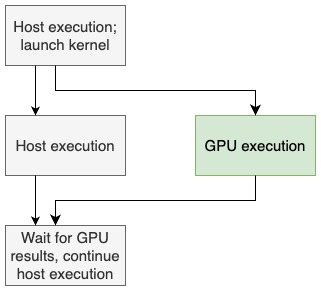
\includegraphics{hostgpuoverlap}
  \caption{Host and device activity}
  \label{fig:hostgpuoverlap}
\end{figure}
Normally, host and device actions can take place concurrently;
see figure~\ref{fig:hostgpuoverlap}.

The `triple chevron' syntax indicates how many blocks, and how many threads per block,
are used to launch the kernel.
You can put a 2D or 3D structure on the blocks by using the \indexcudashow{dim3}
coordinate structure:
\cudaverbatimsnippet{cuhello2use}
The coordinate of the block and the thread within the block can now be
found through the \indexcudashow{blockIdx} and \indexcudashow{threadIdx}
coordinates, which are implicitly defined in each kernel.
\begin{lstlisting}
__global__ helloij() {
  printf("Hello from thread %d in block %d\n",
         threadIdx.x,blockIdx.x);
}
\end{lstlisting}

We give a translation between loop parallelism
and CUDA parallelism.

\begin{block}{Loop code and CUDA code}
  \label{sl:cuda-loop}
\begin{multicols}{2}
\begin{lstlisting}
float *x;
for ( blockIdx_x < gridsize )
  for ( threadIdx_x < blocksize )
    size_t linear = threadIdx_x
      + blockIdx_x * blocksize;
    f( x[linear] );
\end{lstlisting}
\columnbreak
\begin{lstlisting}
__global__ cu_f( float x) {
  size_t linear = threadIdx_x
      + blockIdx_x * blocksize;
  f( x[linear] );
}  

float *x; // on device
cu_f<<<gridsize,blocksize>>>(x);
\end{lstlisting}
\end{multicols}
\end{block}

\Level 1 {Host and device}

Analogous to how OpenMP marked certain regions as parallel,
a \ac{CUDA} program marks certain function calls as
executable on a device.
\begin{itemize}
\item Host: the CPU where the execution starts
\item Device: one of possibly several attached \acp{GPU}.
\end{itemize}
Device code is recognizable by a keyword prefix,
\begin{itemize}
\item
  \indexcudashow{__global__} indicates a function that can be called from the host,
  or recursively from the device;
\item  \indexcudashow{__device__} functions can only be called from the device;
\item \indexcudashow{__host__} marks host code, but that's the default,
  so this keyword is optional.
\end{itemize}

Declare a device function:
\begin{lstlisting}
__global__ void some_cuda_function( /* parameters */ );
\end{lstlisting}
Device code needs have type \lstinline{void}:
return results have to be passed explicitly through memory.

\Level 0 {Host vs device memory}

The host and device have separate memory, so you may need to
synchronize host data to the device.
The mechanism for that depends on how your memory was allocated.

\begin{figure}[ht]
  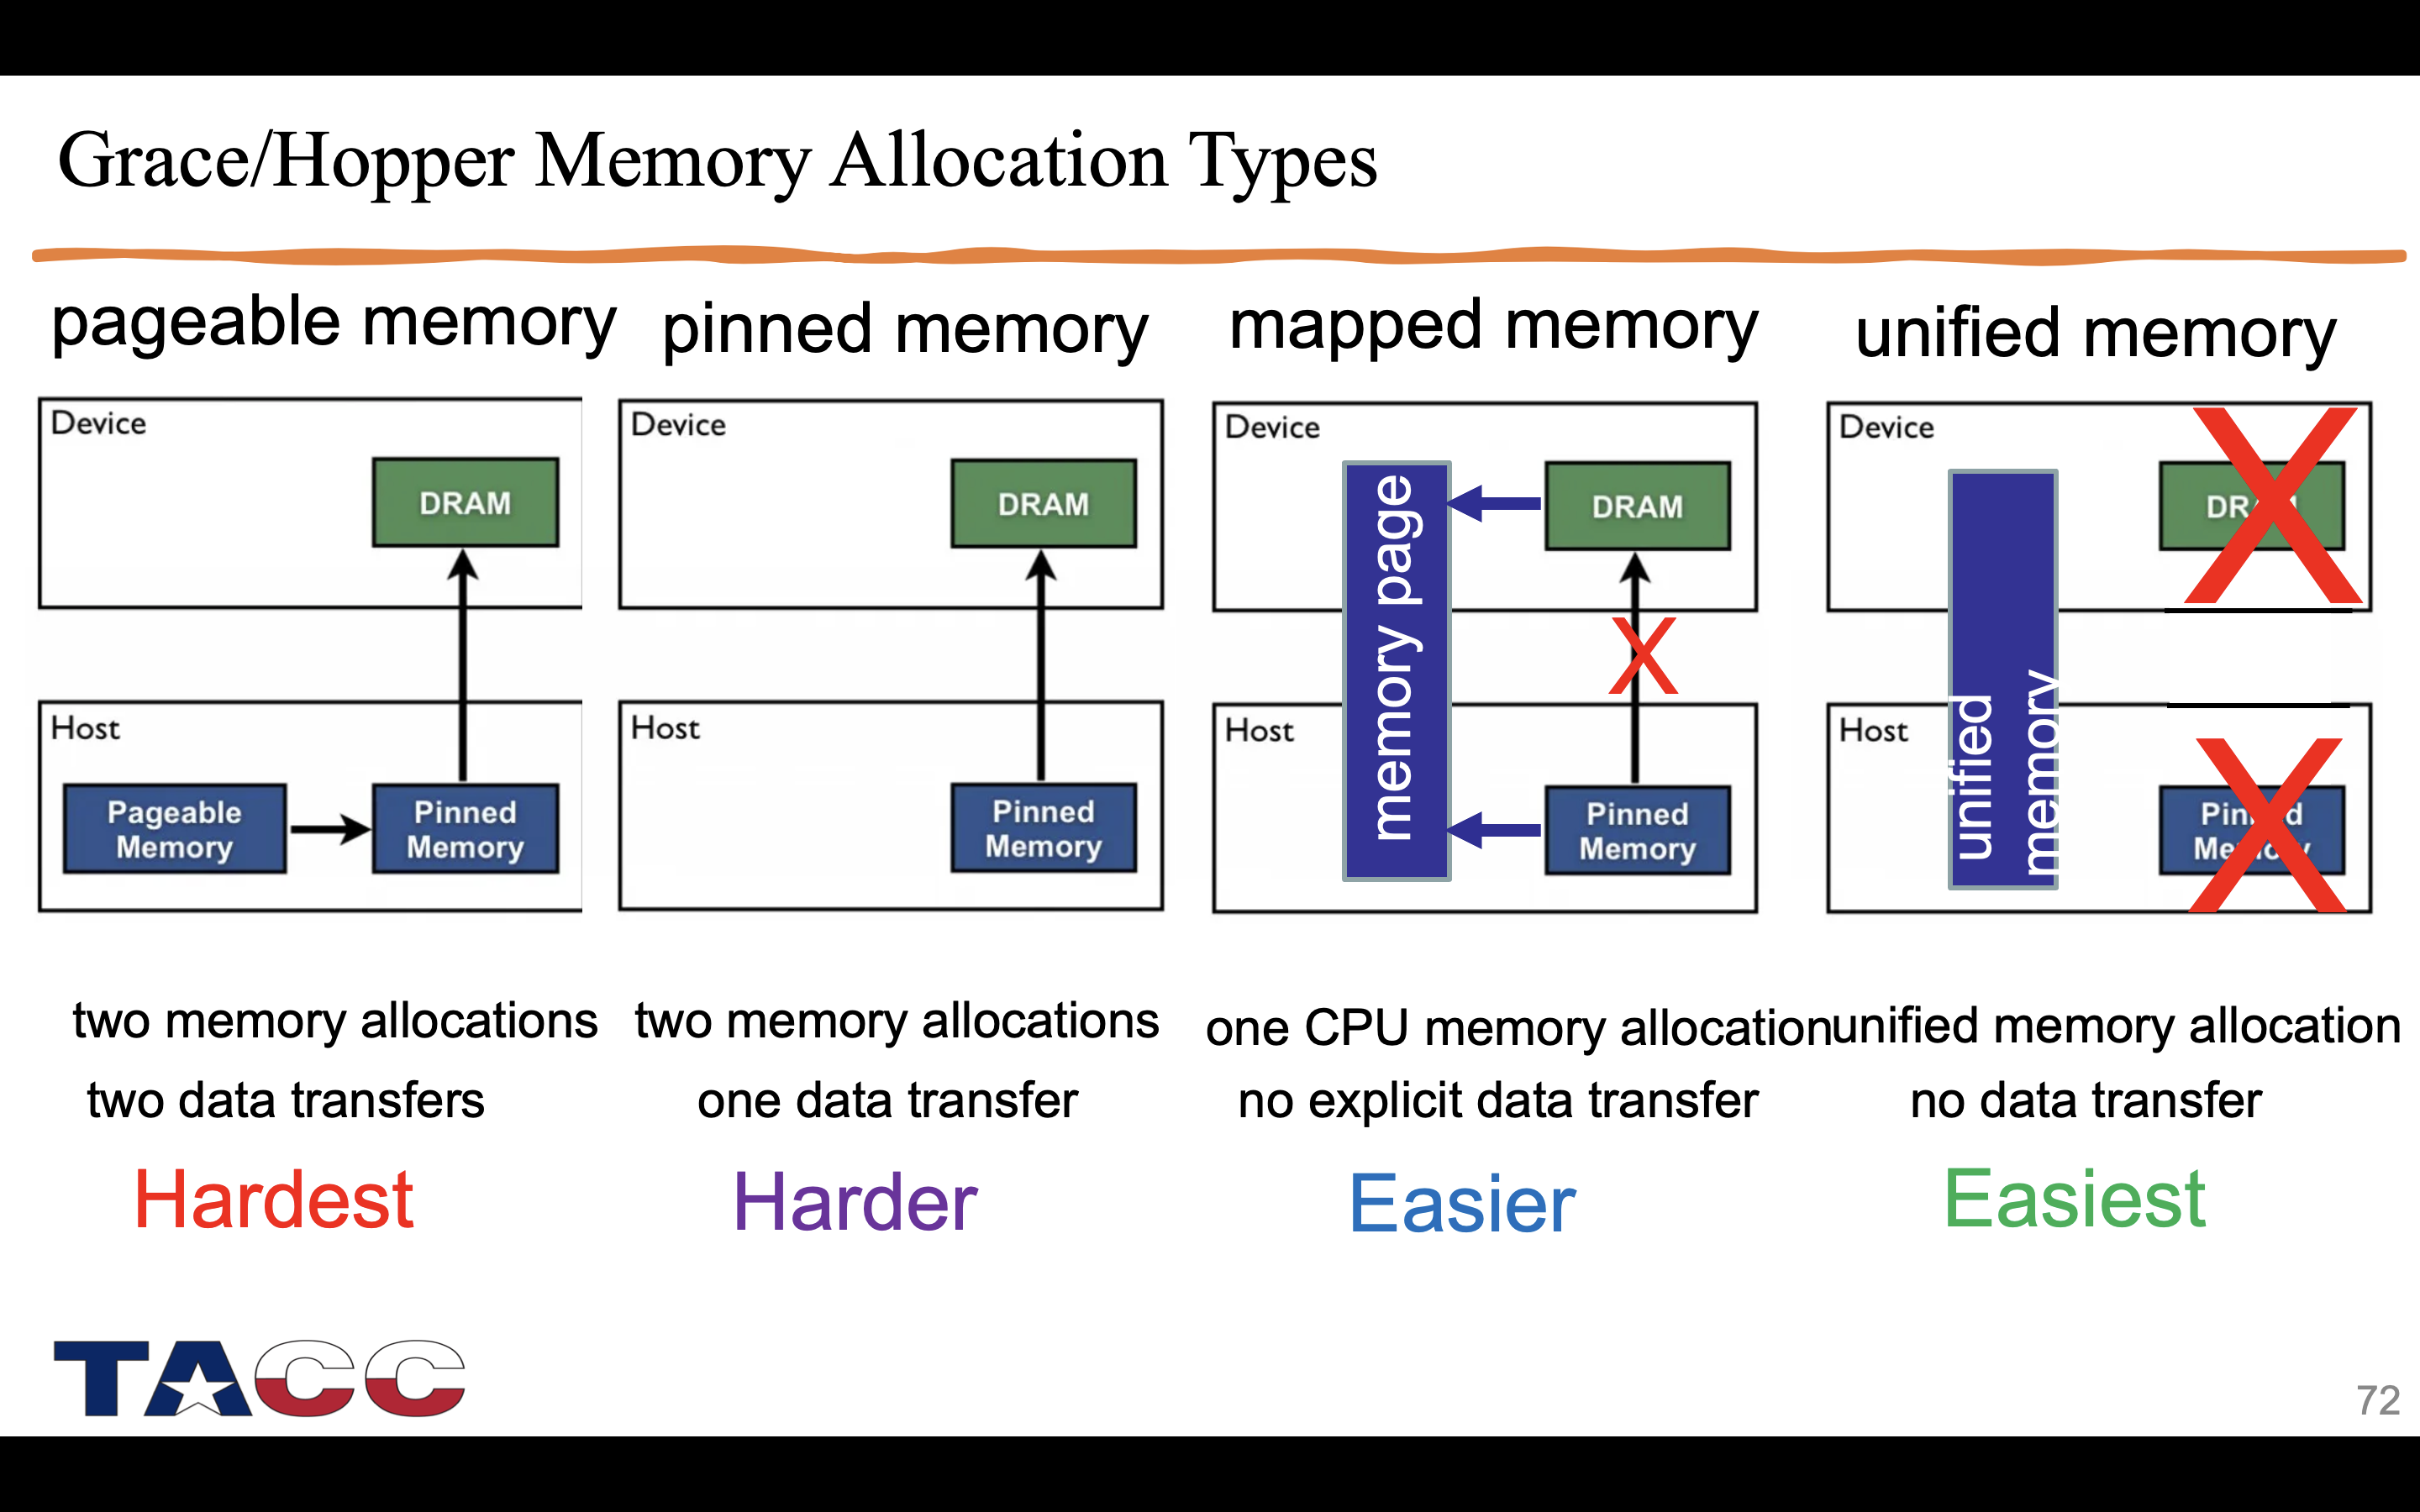
\includegraphics[scale=.15]{gpu-memory-types}
  \caption{Host and device memory coherence}
  \label{fig:cu-memory-types}
\end{figure}
Figure~\ref{fig:cu-memory-types} illustrates these types
and the coherence mechanisms between them.

\Level 1 {Explicit data transfer}

One strategy is allocate data separately for host and device.

Host memory can be traditionally allocated with \lstinline{malloc}
or \indexcudashow{cudaMallocHost}.
The first type is traditional \indextermsub{swappable}{memory};
the second type is \indextermsub{pinned}{memory},
and is permanently resident in memory.
The function \indexcudashow{cudaHostAlloc} behaves like \lstinline{cudaMallocHost}
by default, but has additional flags.

Device memory is allocated with \indexcudashow{cudaMalloc}.
While the resulting pointer is visible to the host code,
the actual memory is on the device and you need copy host data explicitly
between host and device with \indexcudadef{cudaMemcpy}.
This transfer can be between host and device in either direction,
or between two devices.

Allocate input data and copy host values:
\cudaverbatimsnippet{cuhost2devcpy}
After the kernel execution copy output data back:
\cudaverbatimsnippet{cudev2hostcpy}

\begin{lstlisting}
cudaMemCpy( dest_ptr, orig_ptr, byte_size, direction );
// direction:
cudaMemcpyHostToDevice
cudaMemcpyDeviceToHost
cudaMemcpyDeviceToDevice
\end{lstlisting}

Example. We start by allocating host and device memory.
In this case we use regular swappable host memory.
\cudaverbatimsnippet{cuhostdevalloc}

The data is then copied to the \ac{GPU}:
\cudaverbatimsnippet{cudatacopyin}
and after the kernel execution the resulting data is copied back:
\cudaverbatimsnippet{cudatacopyout}

Finally we free host and device memory:
\cudaverbatimsnippet{cumemfreehostdev}

\Level 1 {Implicit transfer}

It is possible create \indextermsub{mapped}{memory}:
host memory that can be mapped to the device.
This is allocated on the host with \indexcudashow{cudaHostAlloc}
using a flag of \indexcudashow{cudaHostAllocMapped}.
The device can then access this memory through a pointer
obtained by \indexcudashow{cudaHostGetDevicePointer}.

This type of memory probably had advantages when \acp{GPU} had far less memory
than the host: it allowed them fast access to host memory.
With current large GPU memories this is less important.
One disadvantage of this mode is that the memory can not be swapped out:
it is \emph{pinned}\index{memory!pinned}\index{pinned memory|see{memory, pinned}}.

You can also allocate \indextermsub{managed}{memory} with \indexcudashow{cudaMallocManaged}.
This type of memory can be written on the host,
but accessed from the device, or the other way around.
The actual mechanism that moves data back and forth
is based on \indexterm{paging}.
\cudaverbatimsnippet{cumanagedalloc}

Also \indexcudashow{cudaHostAlloc}, \indexcudashow{cudaFreeHost}.
\begin{lstlisting}
cudaError_t cudaHostAlloc
   ( void **pHost,size_t count,unsigned int flags );
\end{lstlisting}
Flag values:
\begin{lstlisting}
cudaHostAllocDefault
cudaHostAllocPortable
cudaHostAllocWriteCombined
cudaHostAllocMapped
\end{lstlisting}

\indexcudashow{cudaHostGetDevicePointer}

May require \lstinline{deviceProp.canMapHostMemory}.

\Level 1 {Coalesced memory access}

\Level 0 {Kernels}

You have seen the basic design of a grid of blocks,
where each block is a set of threads.
You can query the limits on the size of a block
(section~\ref{sec:cu-properties})
but common values are:
\begin{itemize}
\item
  The $x,y$ sides of the block cannot exceed~$1024$, and the $z$~side
  can not exceed~$64$;
\item the total size of the block is limited to~$1024$.
\end{itemize}

The blocks are distributed among the \acp{SM},
but even a single block can have more threads than
the \ac{SM} has cores, so
there is a further division in \indextermp{warp}.
A~warp is typically 32 threads.

\Level 1 {Thread indexing}

We need a way of identifying which CUDA thread executes a kernel.
Each kernel execution can query the (globally defined) variables
\indexcudadef{blockIdx} and \indexcudadef{threadIdx}.

It is possible to launch a kernel on more threads than
there are data points. In that case, your code could include
\begin{lstlisting}
int global_thread_id = blockIdx.x * blockDim.x + threadIdx.x; // or 2d, 3d variant
if ( global_thread_id >= datasize ) return;
\end{lstlisting}

The thread index is limited by the size of the block, which has
hardware limits; see section~\ref{sec:cu-properties}.

\Level 1 {Beyond linear indexing}

If we work on two-dimensional data, it makes sense to have
a two-dimensional grid/block structure.
We use the \lstinline{.x} component to find the row,
and \lstinline{.y} component for the column;
this is then translated to a linear index:
%
\cudaverbatimsnippet{index2dij}

\begin{figure}[ht]
  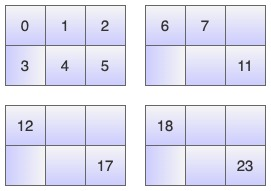
\includegraphics[scale=.8]{cuthreadblock}
  \caption{Two-dimensional thread ordering}
  \label{fig:cu-thread-block}
\end{figure}
In many applications it is enough to know that each thread can
compute the unique location of a data element.
Figure~\ref{fig:cu-thread-block} illustrates the recursive
lexicographic ordering on the threads.

\begin{exercise}
  \label{ex:print2b2}
  Create a two-dimensional array and let each thread write its global number
  in the elemenent where it is active:
  \cudaverbatimsnippet{print2b2write}
  Your program should recreate the layout of figure~\ref{fig:cu-thread-block}.
\end{exercise}

In the above we could also have switched the roles of the \lstinline{x,y} coordinates:
%
\cudaverbatimsnippet{index2dji}

However, this would have performance implications
because of \indextermsub{coalesced}{memory}.

\lstinputlisting[language=shell]{index2d_right.runout}

\lstinputlisting[language=shell]{index2d_wrong.runout}

\Level 1 {Grace Hopper architecture}

\begin{figure}[ht]
  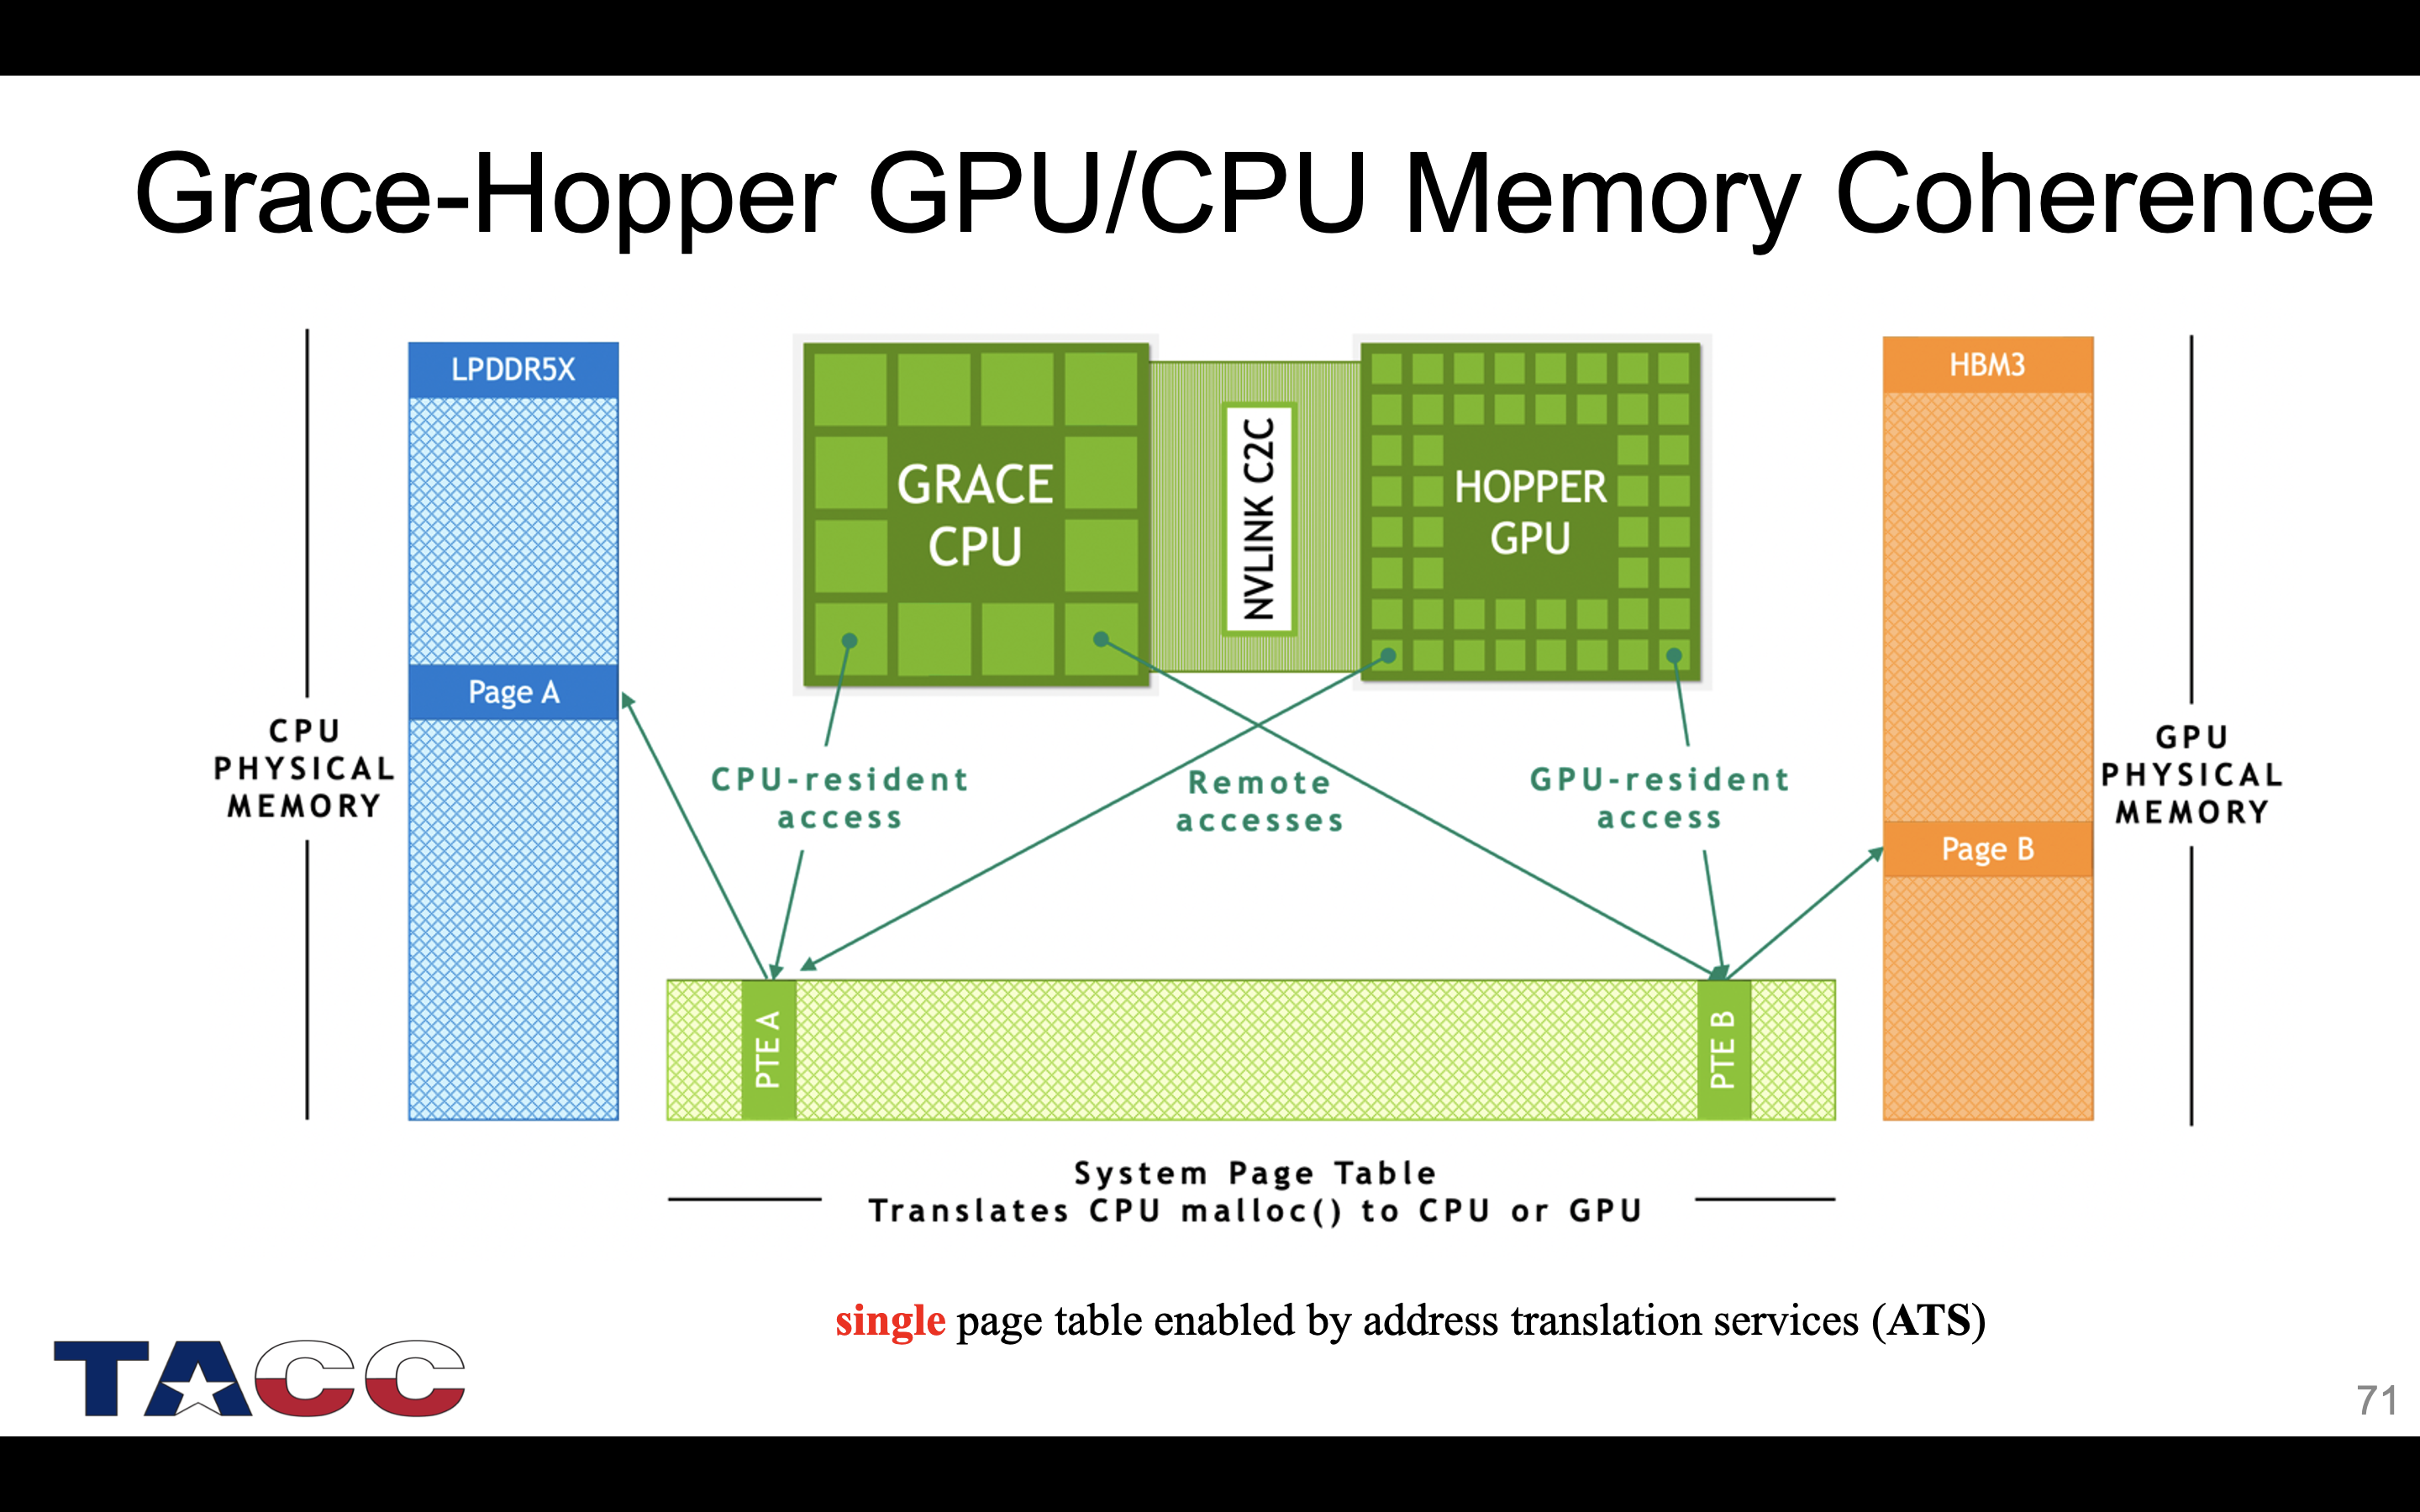
\includegraphics[scale=.15]{grace-hopper-paging}
  \caption{Page table of the Grace Hopper GPU}
  \label{fig:grace-hopper-paging}
\end{figure}
How these memory types are realized on the
\indextermbus{NVidia}{Grace-Hopper}\index{Grace-Hopper (GPU)|see{NVidia, Grace-Hopper}}
GPU architecture is depicted in figure~\ref{fig:grace-hopper-paging}.

\begin{figure}[ht]
  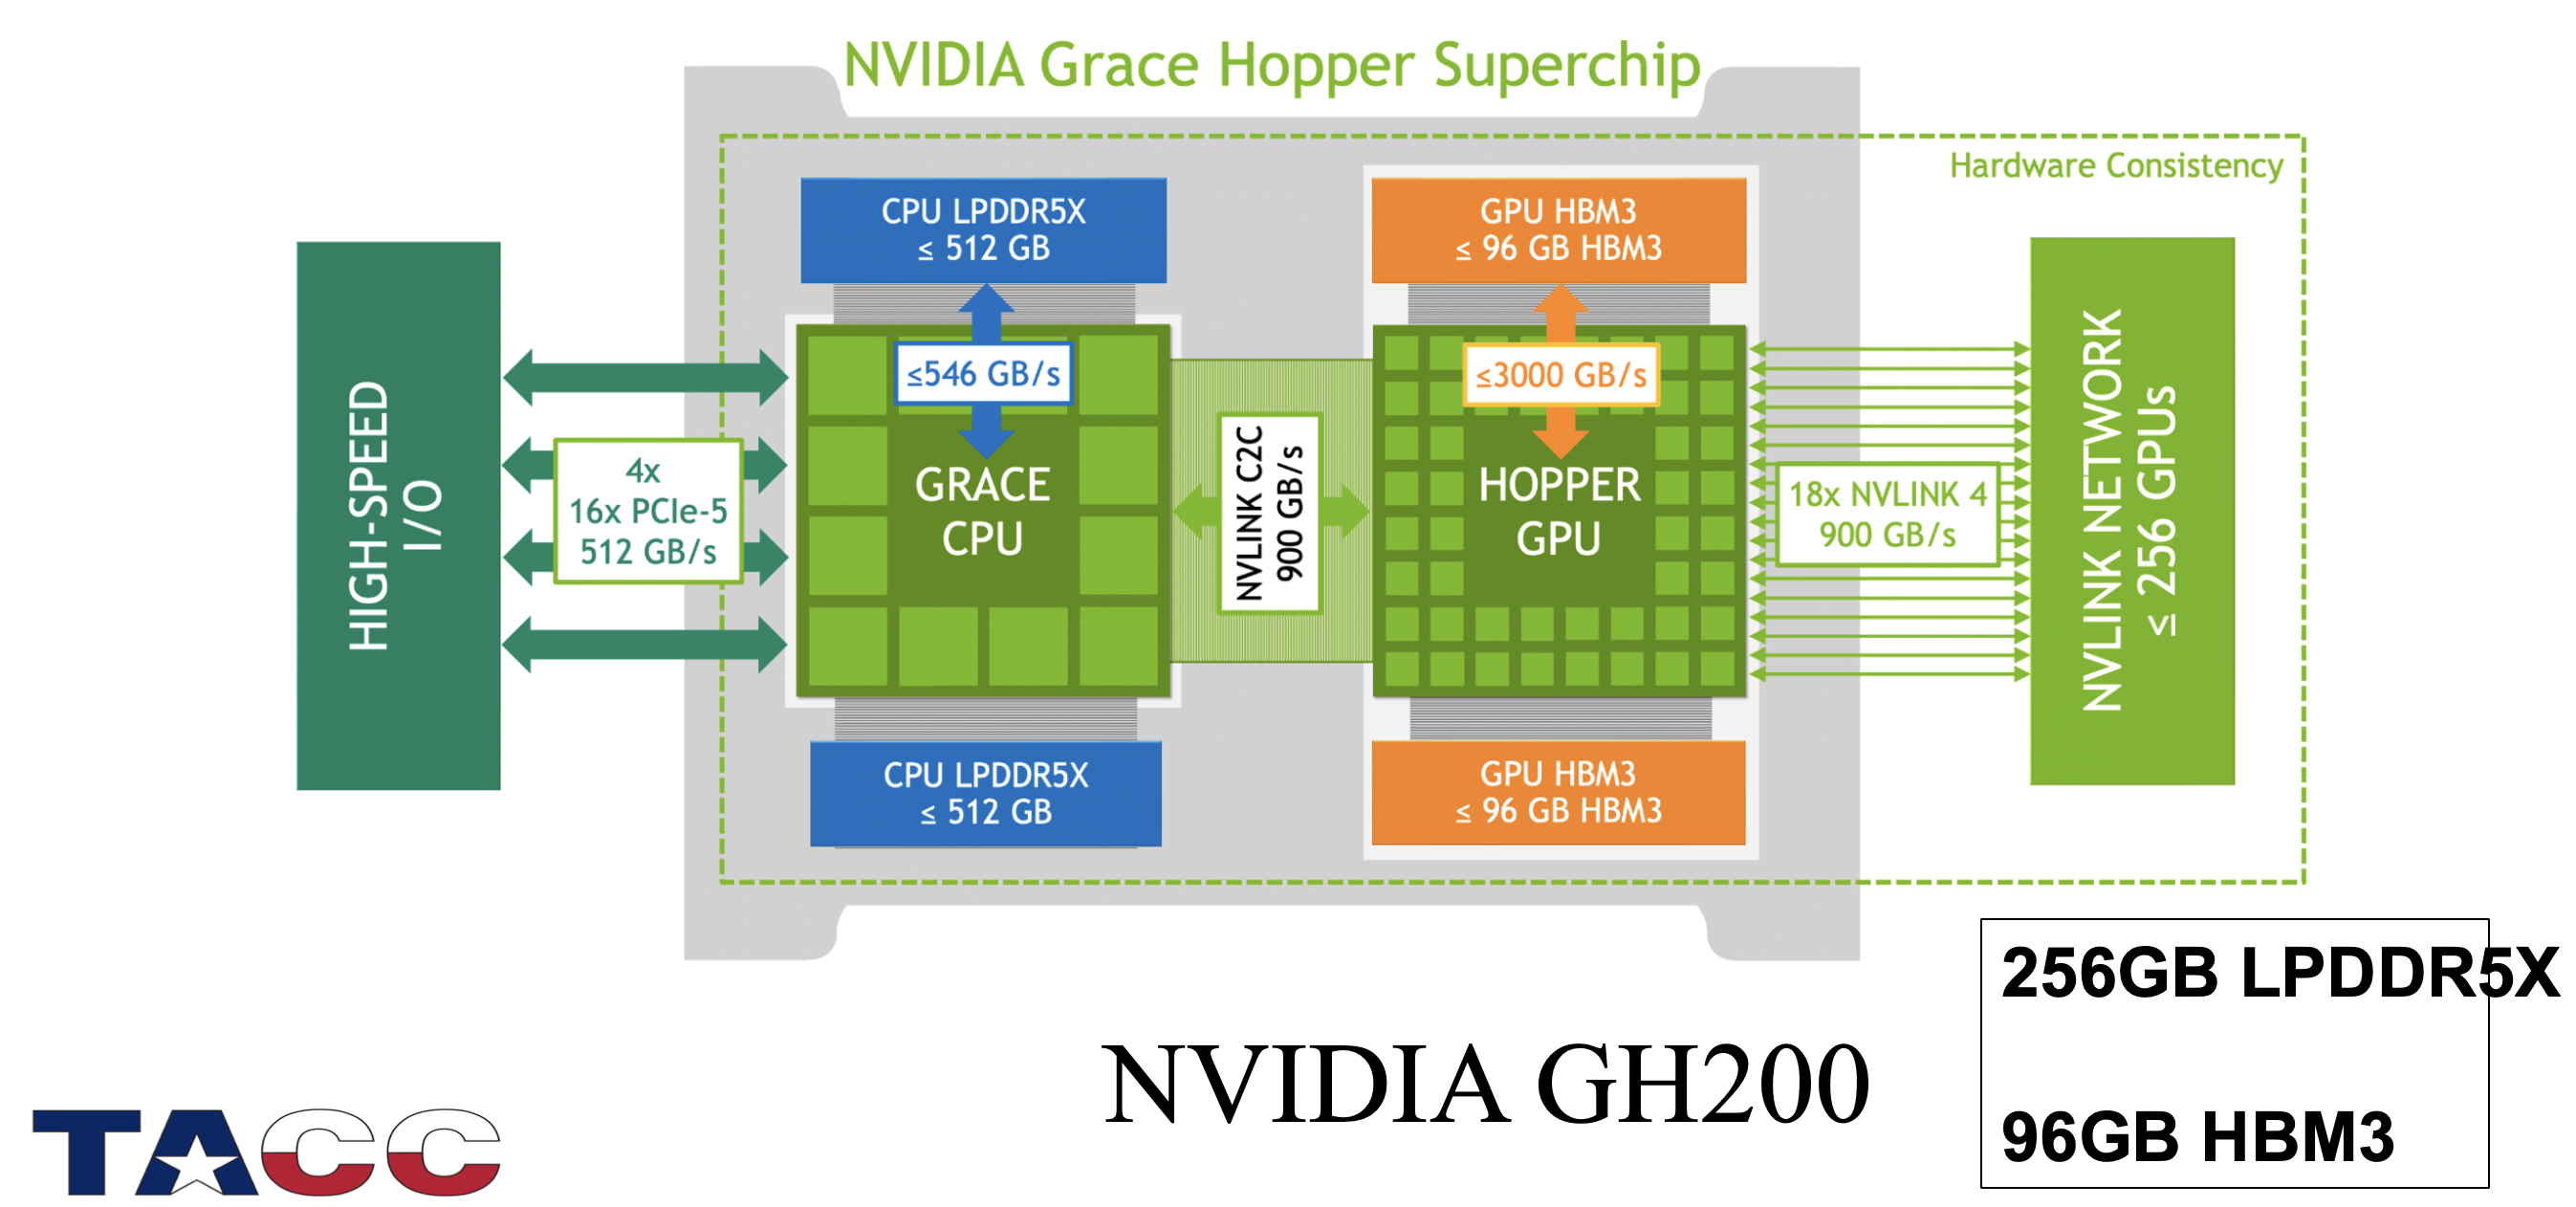
\includegraphics[scale=.15]{grace-hopper-architecture}
  \caption{Hardware diagram of the Grace-Hopper superchip}
  \label{fig:grace-hopper-hardware}
\end{figure}
Hardware specs are given in figure~\ref{fig:grace-hopper-hardware}.

\Level 0 {Device memory}

\Level 1 {Internal structure}

\begin{figure}[ht]
  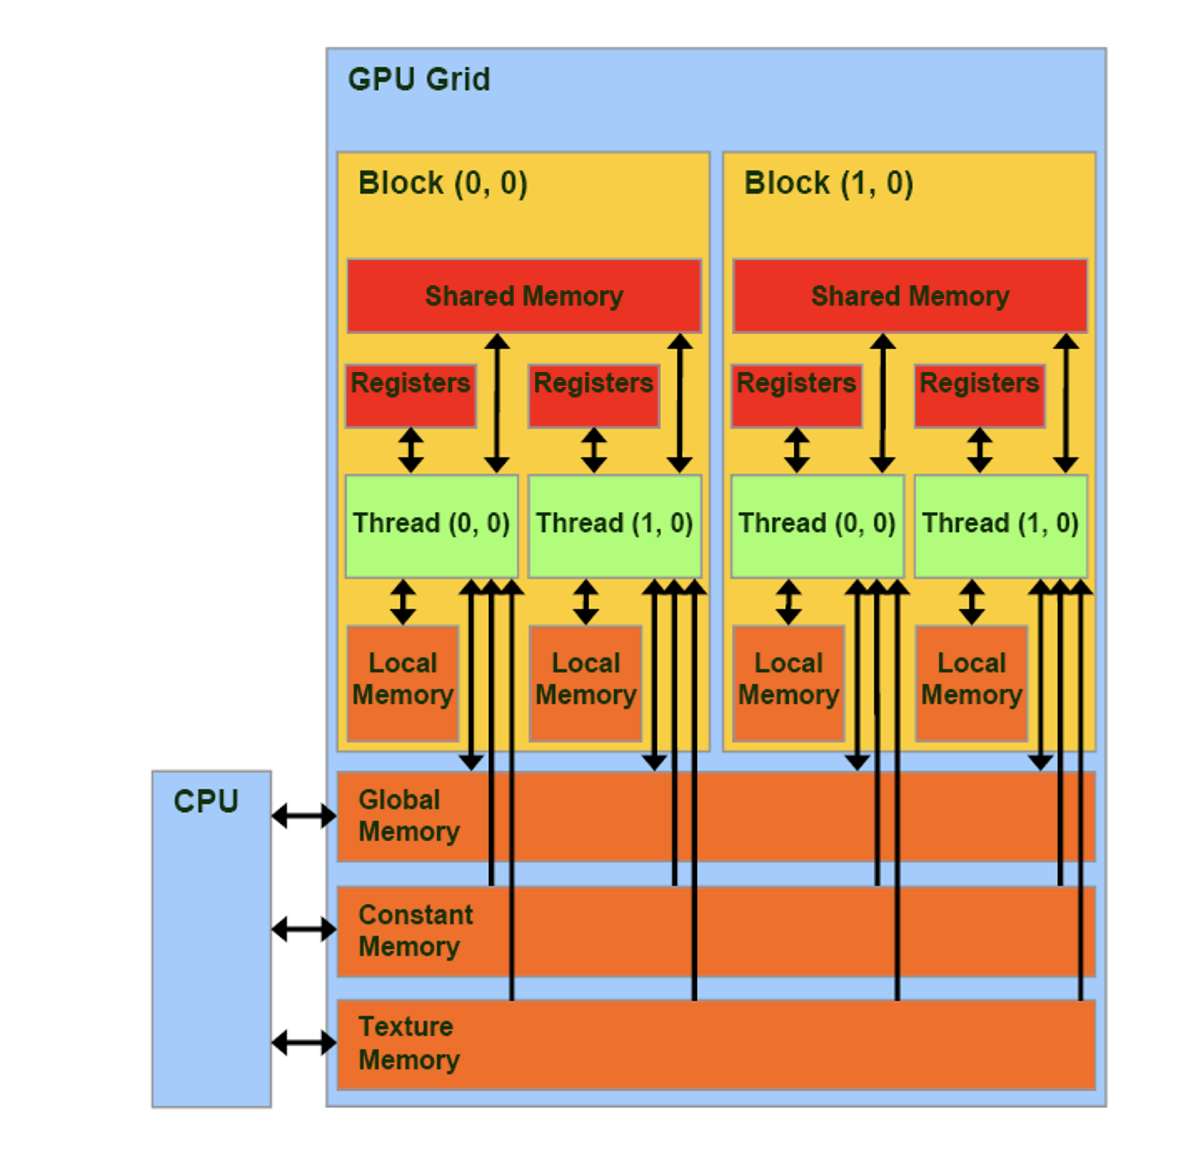
\includegraphics[scale=.3]{gpu-memory-hierarchy}
  \caption{Memory types in a GPU}
  \label{fig:gpu-hierarchy}
\end{figure}
Figure~\ref{fig:gpu-hierarchy} illustrates the different types of
memory inside a GPU.

\Level 1 {Shared memory}

\begin{figure}[ht]
  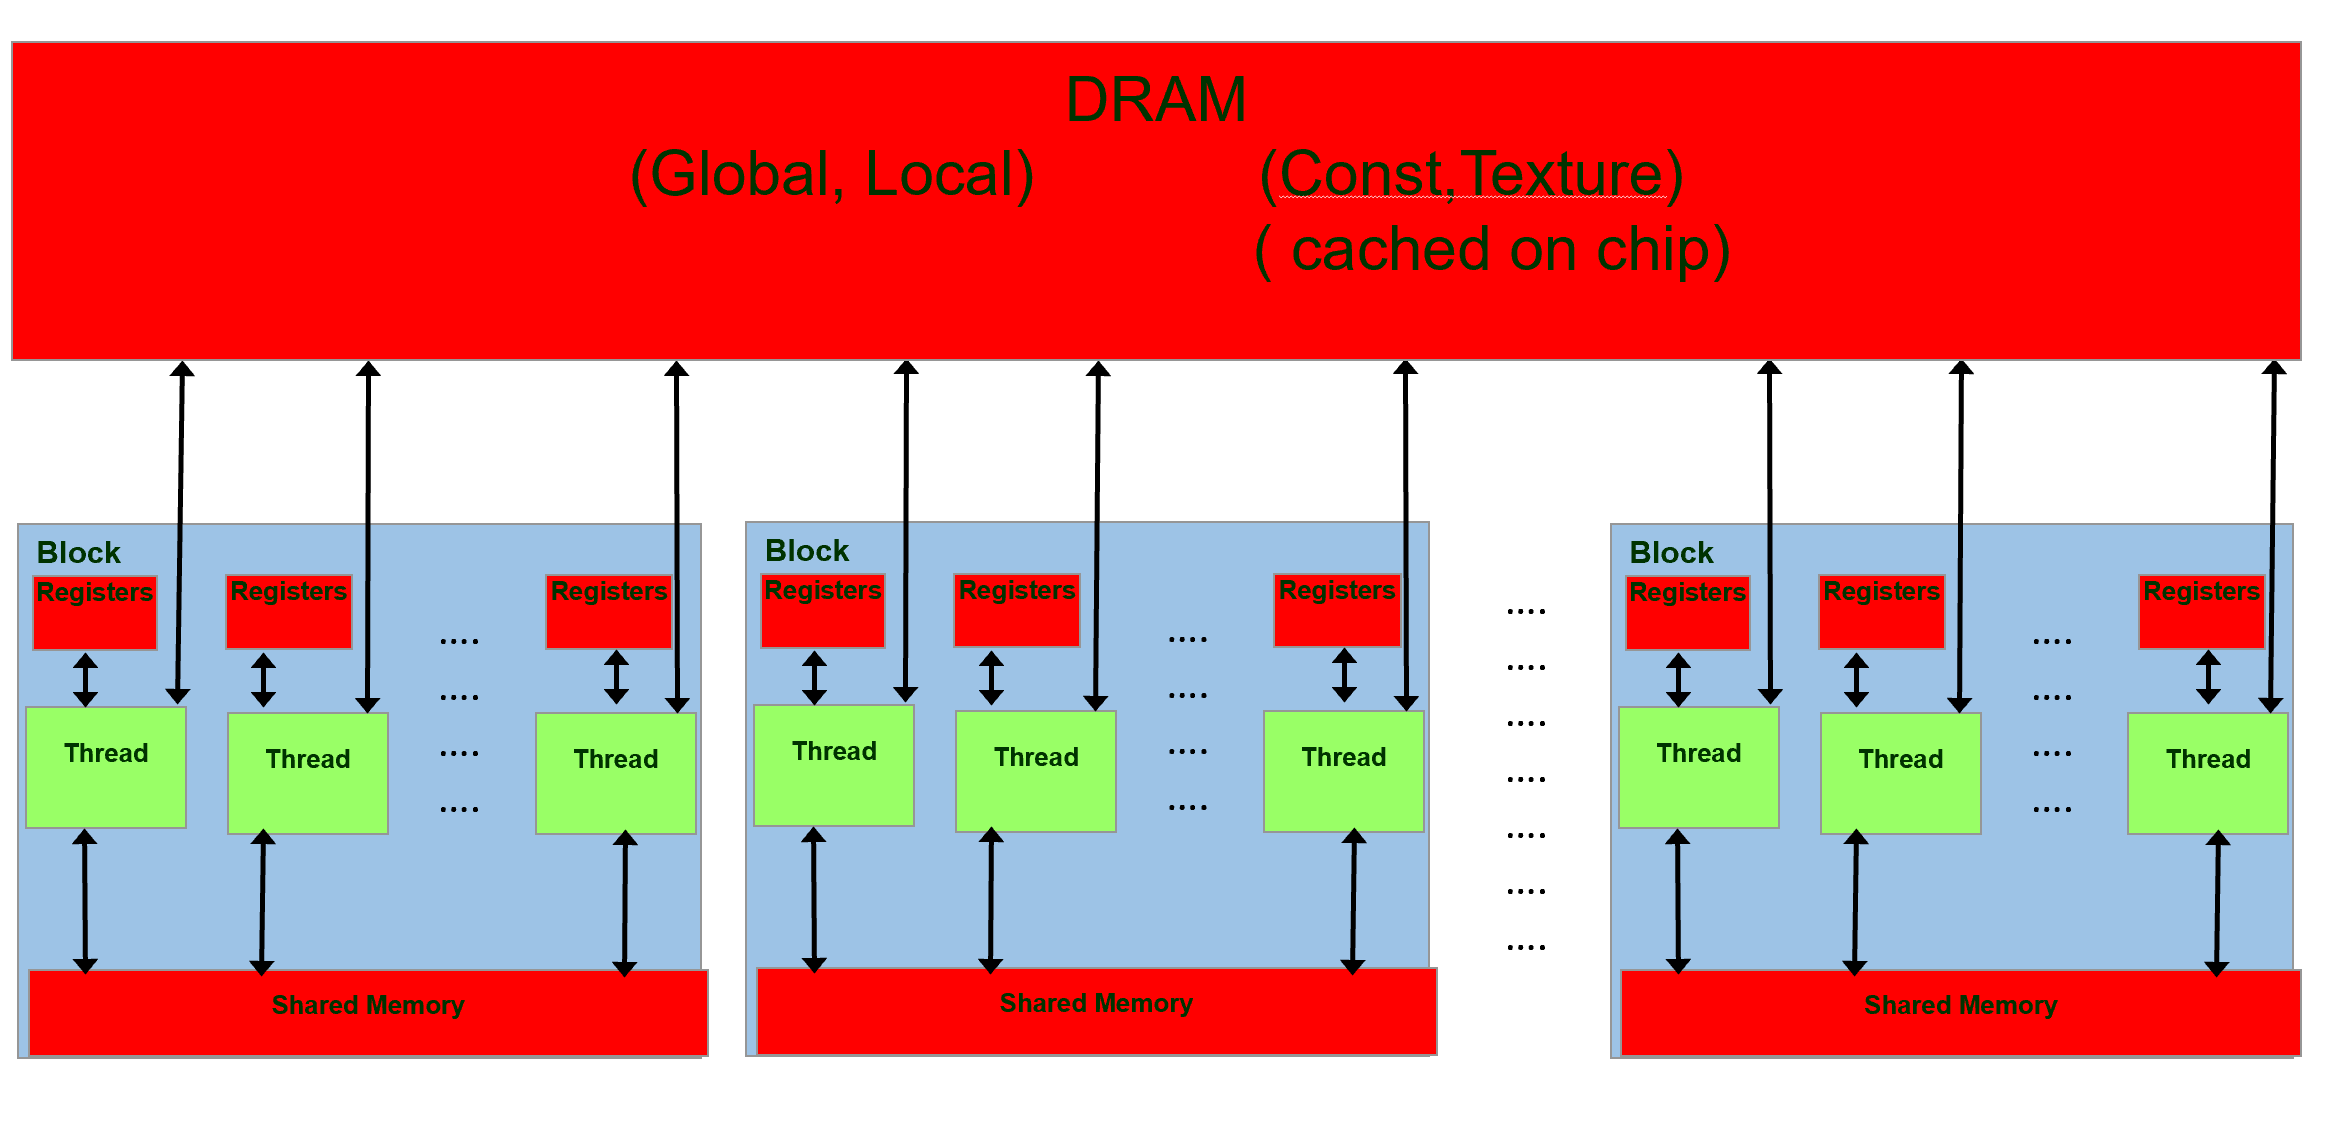
\includegraphics[scale=.6]{nvidia-gpu-memory}  
  \caption{GPU memory structure}
  \label{fig:gpu-memory}
\end{figure}
The way we have coded so far, data is streamed from the
main memory of the \ac{GPU}.
For higher performance it is necessary to use the
\emph{shared memory}\index{memory!shared (GPU)}
of the threads in a block; 
see figure~\ref{fig:gpu-memory}.
This acts like managed cache memory:
data items that are repeatedly accessed
are better copied to shared memory first.

Shared memory is declared by adding the keyword
\indexcudashow{__shared__} to a regular array declaration:
\begin{lstlisting}
__shared__ float tmp[BLOCKSIZE];
\end{lstlisting}

Example five-point stencil.

\Level 0 {Querying}
\label{sec:cu-properties}

Use \indexcudashow{cudaGetDeviceCount} to report how many \acp{GPU} are attached:
\cudaverbatimsnippet{cudevcount}
Possible errors: \indexcudashow{cudaErrorNoDevice} if there are no devices,
and \indexcudashow{cudaErrorInsufficientDriver} if the driver is too old.

Use \indexcudashow{cudaGetDeviceProperties}
to return a \indexcudashow{cudaDeviceProp} object:
\cudaverbatimsnippet{cudevprop}
Here are some of the properties:
\cudaverbatimsnippet{cudevprops}

Blocksize:
\cudasnippetwithoutput{cublockprop}{code/cuda/cxx}{blocksize}

\Level 0 {Synchronization}

\begin{itemize}
\item Threads in a warp are synchronized.
\item Threads in a thread block can be synchronized
  with the \indexcudadef{__syncthreads} function.
\item Thread blocks can not be synchronized.
\item Host and device can be synchronized
  with \indexcudashow{cudaDeviceSynchronize}.
\end{itemize}

\Level 1 {Warp divergence}

The threads in a warp are completely synchronized;
think that they are executed by vector instructions.
This means that conditionals are inefficient.
Code such as
\begin{lstlisting}
if ( threadIdx.%2==0 )
  functionA();
else
  functionB();
\end{lstlisting}
is translated to a sequential execution with masks:
\begin{lstlisting}
bool mask = (threadIdx.x%2==0)
if (mask) functionA();
if (not mask) functionB();
\end{lstlisting}
This differing behavior of the threads inside a warp is known as
\indextermbus{warp}{divergence}.
If at all possible, transform such code
to a mask applied to the on the warps,
rather than the threads.

\Level 1 {Synchronization across blocks}

Fully data parallel operations are relatively easy
as we saw above.
When we start doing reductions we run into the fact that
thread blocks can not be synchronized.
Global reduction operations need synchronization across thread blocks.
This is not easily done. We can either
\begin{itemize}
\item Use atomics;
\item Synchronize outside of CUDA;
\item Use a library.
\end{itemize}

These options are explored for the specific case of reduction operations
in section~\ref{sec:cu-reduce}.

\Level 0 {Performance}

\Level 1 {Timing}

\indexcudashow{cudaEventRecord} acts like a barrier.
So why do we need \indexcudashow{cudaEventSynchronize}?

\begin{lstlisting}
cudaEvent_t start, stop;
cudaEventCreate(&start);
cudaEventCreate(&stop);
float milliseconds = 0.0f;
 
cudaEventRecord(start);
cudaEventSynchronize(start);
// device operation goes here
cudaEventRecord(stop);
cudaEventSynchronize(stop);
cudaEventElapsedTime(&milliseconds, start, stop);
\end{lstlisting}

\Level 1 {Profiling}

\indextermtt{ncu}
\url{https://docs.nvidia.com/nsight-compute/NsightComputeCli/index.html}

\begin{remark}
  Legacy: \indextermtt{nvprof}.
\begin{lstlisting}[language=bash]
nvprof --metrics branch_efficiency your_program
\end{lstlisting}
\end{remark}

Profiler metrics:
\indexcudashow{gld_efficiency},
\indexcudashow{gld_throughput},
\indexcudashow{gld_transactions},
\indexcudashow{gld_transactions_per_request}

\Level 1 {Memory stuff}

\begin{figure}[ht]
  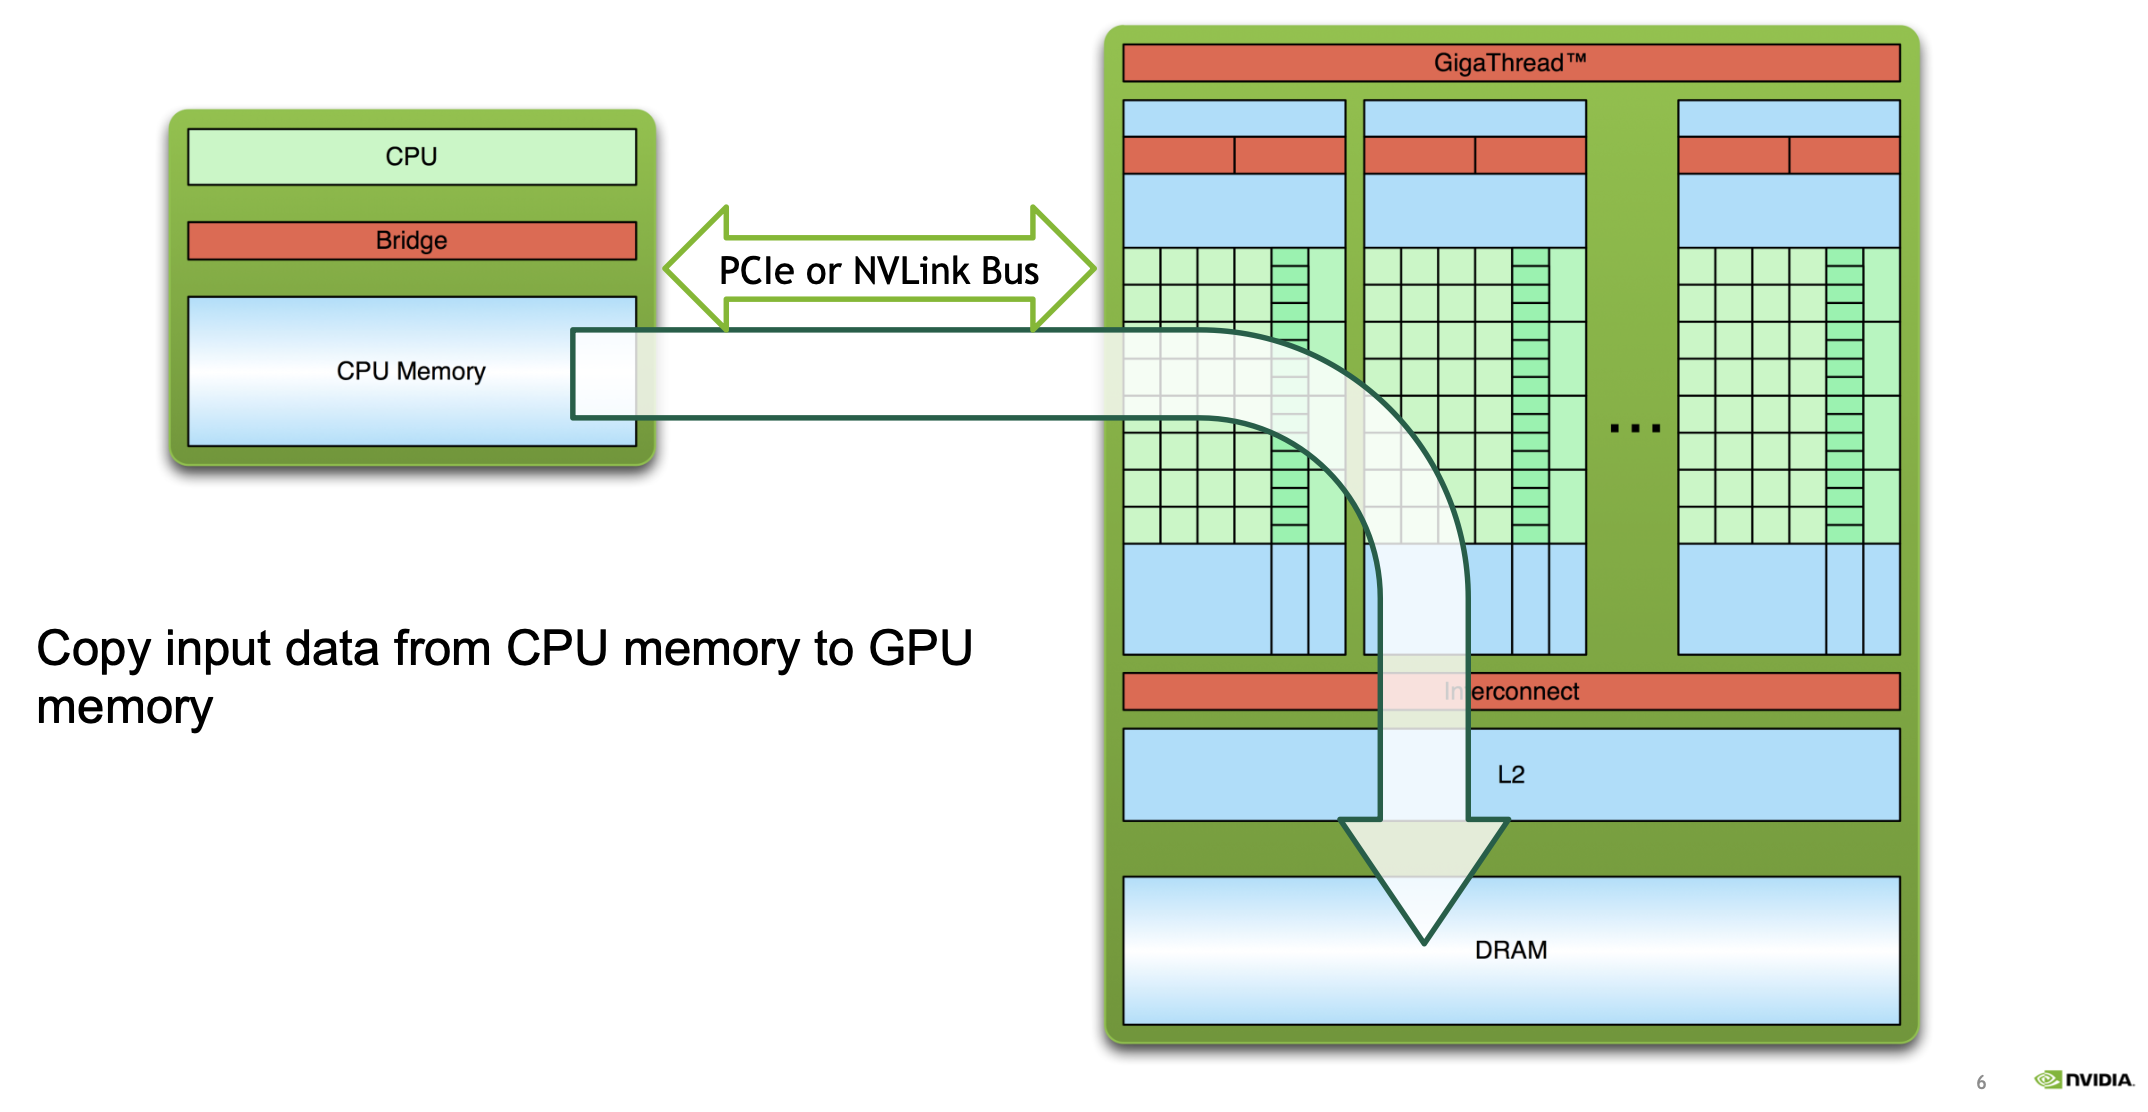
\includegraphics[scale=.4]{GPUcopyfromhost}
  \caption{Memory transfer from host to device}
\end{figure}

%% \begin{figure}[ht]
%%   
\includegraphics[scale=.5]{GPUmemory}
%%   \caption{Structure of GPU memory}
%% \end{figure}

\begin{itemize}
\item Local memory: DRAM.
\item Shared memory: on-chip, shared among thread blocks,
  indicated with \indexcudashow{__shared__}.
\item Constant memory, texture memory, global memory, GPU caches.
\end{itemize}

Variables in global memory by \lstinline{__device__}.

\Level 0 {Reduction}
\label{sec:cu-reduce}

Reduction operations on an indexed set $\{x_i\}$:
\[ r\leftarrow \bigoplus_i x_i \]
are not straightforward since we can not
synchronize between thread blocks.
One solution is to step outside of CUDA.

That means that we call a \ac{CUDA} kernel to reduce
within each threadblock:
\cudaverbatimsnippet{cureductkernelproto}
but follow this up with a summation in the host code:
\cudaverbatimsnippet{cureductoutside}

First of all we use local memory to each thread block,
confusingly called `shared' memory.
\cudaverbatimsnippet{cucopytoshared}

\Level 1 {Implementation 1}

Our first approach is ordinary recursive reduction,
illustrated in figure~\ref{fig:cureduct1}.
\begin{figure}[ht]
  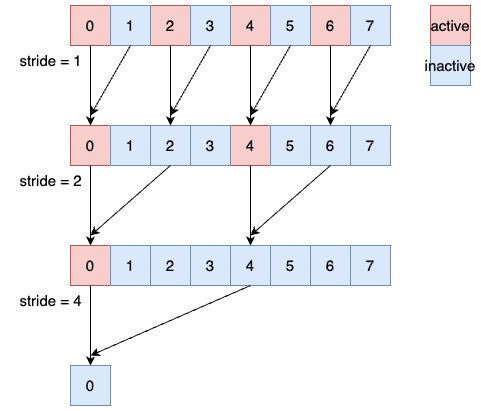
\includegraphics[scale=.6]{reduct1}
  \caption{Recursive reduction}
  \label{fig:cureduct1}
\end{figure}
We let threads
at distances~$2,4,8,\ldots$ sum values
from offsets~$1,2,4,\ldots$.
%%\cudaverbatimsnippet{cureduct1}
\cudaverbatimsnippet{cureductkernel1}

In this approach we recursively eliminate half of all active threads.
The problem here is \indextermbus{warp}{divergence}:
different threads in a warp follow a different control path
through the conditional.

\Level 1 {Implementation 2}

Another approach would be to use a consecutive block of active threads,
and keep all threads in a warp active.
The threads now
address increasingly spaced data;
\begin{figure}[ht]
  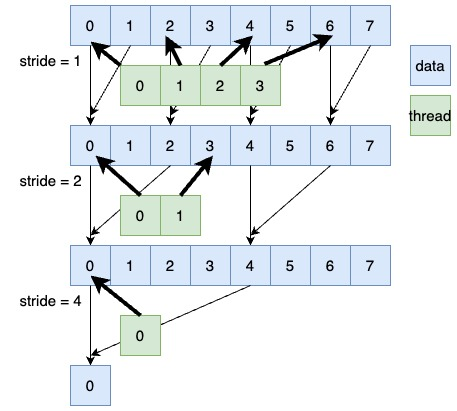
\includegraphics[scale=.6]{reduct2}
  \caption{Recursive reduction with contiguous threads}
  \label{fig:cureduct2}
\end{figure}
see figure~\ref{fig:cureduct2}.
%%\cudaverbatimsnippet{cureduct2}
\cudaverbatimsnippet{cureductkernel2}

Both approaches only do a reduction within a thread block.
Because we can not synchronize between these blocks inside the GPU,
we need a final stage on the host:
\cudaverbatimsnippet{cureductblocks}

\Level 1 {Implementation 3 using Cub}

We can also use the primitives of the Cuda UnBound library
\url{https://github.com/NVIDIA/cccl/tree/main/cub}.
In this case, we use the reduce primitive
with a sum operator:
\cudaverbatimsnippet{cucubreduce}

\Level 0 {Other}
\Level 1 {Dynamic parallelism}

\ac{CUDA} routines can recursively call other
\ac{CUDA} routines.
The recursive call has a grid specification
as on the host.
\begin{lstlisting}
__global__
cuda_fn() {
  if (threadIdx.x%2==0)
    cuda_fn<<<1,blockDim.x/2>>>();
}
\end{lstlisting}

Compile flag: \lstinline[language=bash]{-rdc=true}.

\Level 1 {Asynchronous stream computing}

You can associate a stream number of kernel launches and memory transfers:
\begin{lstlisting}
cudaMemcpyAsync( dest,src,count,kind, stream_number );
kernel_function<<< gridsize,blocksize,memsize,stream_number >>>( arguments );
\end{lstlisting}

Stream creation and destruction:
\begin{lstlisting}
cudaStream_t stream1;
cudaError_t result;
result = cudaStreamCreate(&stream1)
result = cudaStreamDestroy(stream1)
\end{lstlisting}

More fine-grained than \indexcudashow{cudaDeviceSynchronize}
we can use \indexcudashow{cudaStreamSynchronize}\lstinline{(stream)}.
